\documentclass[review,times]{elsarticle}
\usepackage{amsmath,amssymb,amsfonts}
\usepackage{algorithm}
\usepackage{algorithmic}
\usepackage{graphicx}
% Robust figure resolution — works whether pdflatex is invoked from
% references/, repo root, or an Overleaf-style flat upload.
\graphicspath{%
  {figures/}{figures/paper/}{figures/40obj/}%
  {figures/40obj/training/}{figures/40obj/steps/}%
  {references/figures/}{references/figures/paper/}%
  {references/figures/40obj/training/}{references/figures/40obj/steps/}%
  {../docs/figures/}{../docs/figures/paper/}%
  {./}%
}
\usepackage{textcomp}
\usepackage{xcolor}
\usepackage{booktabs}
\usepackage{multirow}
\usepackage{siunitx}
\usepackage{hyperref}
\begin{document}

% =====================================================================
% REVISION 2026-05-15: All ILP-derived numbers in this draft (Tables I,
% II, IV, VI; abstract; §I; §IV-B; §V conclusion; figure captions for
% pareto_n200, runtime_histogram, timing_scaling) have been re-sourced
% from `gnn_ilp_circuit.py` (CP-SAT AddCircuit, no MTZ). Costs are
% exact-solver invariant (verified: max relative delta MTZ↔Circuit
% = 4e-7 across ~6,500 prefix-ILP optima; one 1.6e-5 rounding outlier).
%
% Independent ground-truth at full N via LKH-3 + CP-SAT (Phase 1b):
% 95/95 instances OPTIMAL with LKH-3 tied to CP-SAT on every one.
%
% Phase 2 timing rerun (single machine, PyTorch CUDA build,
% OR-Tools 9.x). Sample sizes match
% v8 captions: N=10/40 use 50 val scenarios, N=200 uses 20.
%
% HARDWARE NOTE: absolute timings on a single machine. After vectorising edge construction
% in the rollout (removed ~40k CPU-GPU syncs per N=200 inference) we measure
% 8.2× LEAP speedup at N=200 (LEAP 0.88 s vs unpruned 7.3 s, mean over 20
% scenarios; cross-run variance is ~15-30% on this small sample because
% CP-SAT timing has heavy tails). The optimality-
% gap claim (max 0.058% at N=200, k=15) reproduces.
%
% Source JSON files:
%   experiments/ilp_timing_circuit_v8.json — Phase 2 timings (unpruned + LEAP)
%   experiments/gap_tables_circuit_v8.json — Phase 3 Table I gap-vs-ILP
%   experiments/gap_table_n10_per_sample_circuit_v8.json — Phase 3 Table II rows
%   experiments/ilp_mtz_vs_circuit_equivalence.json — Phase 1 cost equivalence
%   experiments/results_N{10,40,100,200}_{lkh,cpsat}.json — Phase 1b full-N optima
% =====================================================================

\begin{frontmatter}

\title{Learning-Augmented Exact Optimization for Asymmetric Pick-and-Place Sequencing}

\author[a]{Panav Arpit Raaj\corref{cor1}\fnref{orcid1}\fnref{present}}
\ead{praajarpit@gmail.com}
\author[a]{Atul Thakur\fnref{orcid2}}
\ead{athakur@iitp.ac.in}

\affiliation[a]{organization={BRAIn Lab, Department of Mechanical Engineering, Indian Institute of Technology Patna},
            city={Patna},
            postcode={801106},
            state={Bihar},
            country={India}}

\cortext[cor1]{Corresponding author.}
\fntext[orcid1]{ORCID: \href{https://orcid.org/0009-0001-2476-756X}{0009-0001-2476-756X}}
\fntext[orcid2]{ORCID: \href{https://orcid.org/0000-0001-5937-4793}{0000-0001-5937-4793}}
\fntext[present]{Present address: Robotics Engineer, Eternal.ag.}

\begin{abstract}
We present a learning-augmented exact optimization framework for robotic pick-and-place (PAP) sequencing that combines a graph neural network (GNN) with a constraint programming (CP-SAT) solver. PAP sequencing is an asymmetric travelling salesman problem (ATSP): the travel cost from object $i$ to object $j$ is not equal to the cost from $j$ to $i$ ($c(i,j)\neq c(j,i)$), because the robot's position after handling object $i$ is fixed by the bin assigned to $i$'s type. Standard (symmetric) travelling salesman problem (TSP) methods do not capture this directional cost. A GNN trained by imitation learning on integer linear programming (ILP)-optimal prefixes acts as a \emph{search-space reducer} for the exact solver: rather than replacing optimisation, its logits keep only the top-$k$ outgoing arcs per node, reducing the CP-SAT decision-variable count from $O(N^2)$ to $O(Nk)$. We call the result \textbf{LEAP} (Learning-Enhanced Arc Pruning). At $N{=}200$, LEAP runs $8.3\times$ faster than the unpruned CP-SAT baseline while remaining empirically near-optimal (worst-case gap 0.058\% to the unpruned optimum on our test set); because CP-SAT still solves the pruned arc set exactly, this extends practical exact optimization to larger PAP instances. The graph uses three node types (robot, object, and bin), with a distinct bin node per object type, processed by a standard graph attention network (GAT). Classical metaheuristics give no a priori optimality guarantee, whereas LEAP is solver-backed and consistently near-optimal in our experiments. The AI contribution is a graph-learning arc-pruning method that makes exact constraint solving tractable on larger instances; the engineering application is travel-time-efficient robotic sorting, with direct relevance to warehouse order fulfilment, automated waste and recycling sortation, and conveyor-based assembly kitting.
\end{abstract}

\begin{keyword}
Learning-Augmented Optimization \sep Graph Neural Networks \sep Pick-and-Place Sequencing \sep Robotic Sorting \sep Combinatorial Optimization \sep Asymmetric Travelling Salesman Problem \sep Warehouse Automation \sep Industrial Robotics
\end{keyword}

\end{frontmatter}

%========================================================================
\section{Introduction}
%========================================================================

Pick-and-place (PAP) sequencing is a core planning task in robotic automation: a manipulator must determine the order in which to pick objects from a workspace and deposit them into designated bins so as to minimise total travel time. The problem is NP-hard \cite{chalasani1996}; the $N!$ candidate sequences grow combinatorially, making exhaustive search impractical beyond toy instances. It arises in warehouse bin picking \cite{cheng2024drl}, automated waste sorting \cite{gundupalli2021sequence, kiyokawa2024challenges}, and robotic kitting in manufacturing.

We organise prior methods by their distance from the integer linear programming (ILP) optimum. \emph{Greedy heuristics} are the cheapest ($O(N^2)$) but the most myopic: even the stronger nearest-cycle (NC) variant, which greedily picks the object with the smallest combined pick-then-place leg cost, cannot reason about how the robot's post-placement position affects downstream picks, so its tours are typically several percent above optimal. \emph{Classical metaheuristics} (simulated annealing, tabu search, guided local search) are general-purpose iterative-improvement loops that perturb a candidate tour until a time budget expires; they close most of the gap to the optimum in practice, though without an a priori guarantee on how close they are. \emph{Exact solvers} reach the optimum and prove it, but scale exponentially: beyond $N\!\approx\!100\text{--}200$ objects, even strong formulations (DFJ with lazy subtour cuts \cite{dantzig1954}, global Hamiltonian-circuit constraints) exceed real-time budgets. The open question is therefore not which method is fastest in isolation but which can be both \emph{tractable at scale} and \emph{reliably near-optimal with solver backing}; existing methods tend to offer one or the other. Our framework keeps ILP, the gold-standard exact solver that returns provably optimal tours, as the quality reference and uses a GNN to reduce its search space, improving tractability at larger scales.

We close this gap with a \textbf{learning-augmented exact optimization} framework. A GNN trained via imitation learning on ILP-optimal prefixes serves as a \emph{search-space reducer}: by using GNN logits to retain only the top-$k$ candidate arcs per node, we reduce the underlying CP-SAT solver's decision variable count from $O(N^2)$ to $O(Nk)$. This yields a 8.3$\times$ speedup over the unpruned CP-SAT Circuit solver at $N{=}200$ with worst-case optimality gap of 0.058\%. We verify correctness against Concorde \cite{applegate2006concorde} (via the Jonker--Volgenant ATSP-to-TSP transformation) on small instances.

The framework's value emerges at scale. At small $N$ (${\le}20$), the ILP is already fast and metaheuristics find near-optimal solutions cheaply; the GNN adds little. At large $N$ (${\ge}40$), the ILP becomes intractable and metaheuristics, while producing strong solutions, leave their distance from the optimum unknown. A metaheuristic might achieve 4\% improvement over greedy, but cannot quantify how much further improvement is possible. LEAP bridges this regime: by solving exactly over a learned arc subset, it returns solutions that are empirically within 0.058\% of the unpruned CP-SAT optimum at $N{=}200$ (mean 0.019\%) on our test set, while solving in 0.88\,s, beating both the unpruned exact solver (7.3\,s) and the metaheuristics' fixed 1\,s budget.

Two structural insights enable the GNN. First, PAP is an \emph{asymmetric} TSP: the travel cost between two objects depends on order, $c(i,j)\neq c(j,i)$, because after placing object $i$ the robot sits at bin $b_{\tau(i)}$ (set by $i$'s type), so the cost of reaching $j$ next is governed by $b_{\tau(i)}$ rather than by $o_i$. This asymmetry is invisible to standard TSP methods that embed all nodes as homogeneous 2D coordinates. Second, the pick-and-place action has an inherent \emph{cyclic} structure (robot$\to$object$\to$bin$\to$robot) that we model as a directed graph with three semantically distinct node types.

We make the following contributions:
\begin{enumerate}
    \item \textbf{LEAP} (Learning-Enhanced Arc Pruning), a GNN-guided exact optimization framework in which a GNN prunes the arc space for a CP-SAT circuit solver that then solves exactly over the pruned arcs, achieving 8.3$\times$ speedup over the unpruned solver at $N{=}200$ with an empirical worst-case gap of $<$0.06\% to the unpruned optimum.
    \item A \textbf{task-specific graph formulation of PAP-as-ATSP} with semantically distinct node types (robot, object, bin; one bin per object type) and directed feedback edges, processed using a standard GAT, which allows the network to learn placement-dependent cost asymmetry. The key design decision is the \emph{graph structure}, not the choice of neural architecture: replacing GAT with GCN on the same graph drops gap-vs-greedy from $+2.59\%$ to $-0.51\%$ at $N{=}40$ (Table~\ref{tab:ablations}), confirming that the encoding carries the information.
    \item An \textbf{empirical comparison} against classical metaheuristics (Guided Local Search, Simulated Annealing, 2-opt) and a greedy nearest-cycle baseline, showing that all three metaheuristics produce strong solutions within a 1\,s budget with no a priori optimality guarantee, whereas LEAP provides solver-backed solutions that are empirically near-optimal at scale.
    \item A \textbf{$k$-sensitivity analysis} characterising the quality--speed Pareto frontier of the arc pruning, showing $k{=}15$ as the sweet spot across problem sizes.
    \item An \textbf{analysis of why arc pruning was substantially more effective than warm-start hinting} for this problem class under the evaluated solver configurations, with four negative results showing that providing GNN solutions as solver hints gave limited benefit in our experiments, whereas arc pruning provided substantial speedup, consistent with the Neural Diving insight \cite{nair2021neural} that the network's value lies in shrinking the problem, not bounding it.
\end{enumerate}

The remainder of this paper is organised as follows. Section~\ref{sec:lit} reviews related work. Section~\ref{sec:methods} presents the problem formulation, graph representation, GNN architecture, and training. Section~\ref{sec:ilp_accel} describes the LEAP framework. Section~\ref{sec:data} describes the dataset. Section~\ref{sec:results} reports results, ablations, and analysis. Section~\ref{sec:conclusion} concludes.

%========================================================================
\section{Literature Review}\label{sec:lit}
%========================================================================

\subsection{PAP Sequencing and Its Relation to TSP}

PAP shares combinatorial structure with TSP \cite{dantzig1954}, but is structurally richer: TSP involves a single homogeneous node type and symmetric costs, while PAP has three entity types (robot, object, bin) and asymmetric cycle costs. Collapsing PAP to TSP by treating each object as a city discards the bin assignment and falsely assumes the cost of visiting object $i$ then $j$ is independent of which bin $i$ was deposited in. Han, Feng, and Yu \cite{han2020pap} formally prove greedy variants are suboptimal in conveyor PAP and demonstrate 10--40\% efficiency loss versus dynamic programming on SCARA and Delta robots. PAP also shares structure with pickup-and-delivery problems \cite{savelsbergh1995pdp} and the Stacker Crane Problem \cite{frederickson1978sc}, both of which pair pickup and dropoff actions on a graph; LEAP differs in that bin destinations are determined by object type rather than freely matched, so the asymmetric cycle cost is fully determined by the chosen pick rather than by an additional assignment decision.

\subsection{Classical Metaheuristics}

Simulated annealing (SA) \cite{kirkpatrick1983sa} and tabu search \cite{glover1989tabu} are general-purpose metaheuristics widely applied to TSP and ATSP. Guided local search (GLS) \cite{voudouris2003gls} augments local search with penalty-based diversification. The Lin--Kernighan--Helsgaun (LKH) heuristic \cite{helsgaun2000lkh} achieves near-optimal results on symmetric TSP but requires adaptation for ATSP. All these methods provide no a priori optimality guarantee: absent an exact reference, their distance from the optimum is uncertified. Our framework uses the OR-Tools implementation \cite{ortools} of these metaheuristics as baselines; they produce strong solutions, but with no a priori optimality guarantee, whereas LEAP provides solver-backed solutions that are empirically near-optimal in our experiments.

\subsection{Greedy Methods and Their Limits}

The nearest-neighbour heuristic \cite{rosenkrantz1977} runs in $O(n^2)$ with a worst-case $\Theta(\log n)$ approximation ratio. In PAP, the stronger \emph{Nearest Cycle} (NC) variant selects the object minimising the full pick-and-place step cost $\lVert r_t - o_i \rVert + \lVert o_i - b_{\tau(i)} \rVert$. NC accounts for the placement leg but remains myopic. Throughout this paper, our greedy baseline refers to NC; improvements over NC are harder to achieve than over basic nearest-neighbour.

\subsection{Neural Combinatorial Optimisation}

Vinyals et al.\ \cite{vinyals2015pointer} introduced Pointer Networks for combinatorial sequencing. Kool et al.\ \cite{kool2019attention} replaced the LSTM encoder with a Transformer, achieving state-of-the-art TSP results via REINFORCE. POMO \cite{kwon2020pomo} and Sym-NCO \cite{kim2022symnco} exploit TSP symmetries (start-node invariance, rotation/reflection) that do not hold in PAP. Costa et al.\ \cite{costa2020learning2opt} trained an RL agent for 2-opt. Perera et al.\ \cite{perera2023gpn} combined a GNN encoder with a Pointer Network decoder for TSP. All these methods operate on homogeneous graphs of 2D coordinates; semantically distinct node types and asymmetric cycle costs are not addressed, making direct application to PAP non-trivial.

We do not evaluate these neural TSP solvers empirically against LEAP for three structural reasons. First, PAP costs are \emph{asymmetric and node-type-dependent}: the travel cost from object $i$ to object $j$ depends on bin assignment $b_{\tau(i)}$, so the input cannot be represented as a symmetric distance matrix over 2D coordinates. Second, the graph has \emph{three semantically distinct node types} (robot, objects, bins) with typed edges that carry information unavailable in standard TSP encoder inputs. Third, all published neural TSP solvers are trained on symmetric 2D Euclidean instances with uniform node types; their architectures and any pre-trained weights do not transfer to PAP. Training a Pointer Network or Attention Model from scratch on PAP would require dataset construction and hyperparameter search comparable to this work's GNN, while still leaving its distance from the optimum unquantified. LEAP instead uses the GNN \emph{only} to reduce the arc space for an exact solver, which then solves the pruned sub-problem exactly; the resulting optimality is over this reduced arc set rather than the original unrestricted problem.

\subsection{GNNs for Combinatorial Optimisation}

Cappart et al.\ \cite{cappart2023gnnco} argue that GNNs are the natural architecture for combinatorial optimisation due to permutation invariance, sparsity awareness, and flexibility for richer node types. Chung et al.\ \cite{chung2025ncosurvey} identify industrial sequencing as an underexplored NCO domain requiring structural modification beyond standard TSP.

\subsection{Learning-Augmented Exact Solvers}

Nair et al.\ \cite{nair2021neural} introduced Neural Diving alongside Neural Branching: Neural Diving uses a neural network to produce partial integer-variable assignments that fix some variables, yielding a smaller residual sub-MIP for a downstream exact solver. We adopt this \emph{partial-assignment philosophy} and apply it at the arc level: rather than hinting the solver with a candidate tour (which we show in Section~\ref{sec:hint_fail} provides negligible benefit because hints only bound the incumbent), we use GNN logits to eliminate low-probability arcs and shrink the solver's decision space directly. Khalil et al.\ \cite{khalil2016learning} learned branching policies for branch-and-bound; Gasse et al.\ \cite{gasse2019exact} trained GNNs to imitate strong branching decisions. Closer in spirit to our arc-pruning step is the learning-to-sparsify line of work: Sun, Lauri, and Dutta \cite{sun2021sparsify} train an ML model to prune $>$85\% of TSP edges as preprocessing before exact ILP while preserving most optimal-tour edges. Edge-heatmap methods produce per-edge probabilities used to constrain or guide subsequent search: Joshi, Laurent, and Bresson \cite{joshi2019gcntsp} via a GCN, Fu, Qiu, and Zha \cite{fu2021gentsp} via a generalisation framework, and Min, Bai, and Gomes \cite{min2023utsp} unsupervised. For asymmetric instances specifically, MatNet \cite{kwon2021matnet} is the closest pure-neural ATSP solver. These methods all operate on homogeneous graphs of city coordinates and produce tours autoregressively or via beam search; LEAP differs by (i) supporting three semantically distinct node types with type-dependent asymmetric costs over a heterogeneous cycle topology and (ii) handing the pruned arc set to a CP-SAT circuit solver that solves it exactly, so the solver's optimality holds over the surviving (pruned) sub-problem rather than the full arc set.

%========================================================================
\section{Methods}\label{sec:methods}
%========================================================================

We formulate PAP sequencing as a sequential decision process and train a GNN policy via imitation learning on ILP-optimal prefixes.

\subsection{Problem Formulation and Cost Model}

We consider a planar PAP task in a $W \times W$ workspace ($W=100$). At each step $t$, the agent selects one remaining object $a_t$ to pick and place into its assigned bin. The robot starts at $r_0 \in \mathbb{R}^2$ and updates its pose to the bin location after each placement. The step cost is:
\begin{equation}
c_t = \lVert r_t - o_{a_t} \rVert_2 + \lVert o_{a_t} - b_{\tau(a_t)} \rVert_2,
\end{equation}
where $o_{a_t}$ is the object position and $b_{\tau(a_t)}$ is the target bin for object type $\tau(\cdot)$. The objective is to minimise total cost $C = \sum_{t=1}^{N} c_t$.

The cost is \emph{asymmetric}: picking object $i$ then $j$ costs differently from picking $j$ then $i$, because the robot's position after placing $i$ is the bin $b_{\tau(i)}$, which depends on $i$'s type. Concretely, if a red object's bin is in the top-left corner and a blue object's bin is in the bottom-right, the robot ends up in very different positions depending on which it picks first. This type-dependent asymmetry is invisible to standard TSP formulations that treat all nodes as interchangeable 2D coordinates. For $N$ objects the search space is $N!$. The Held--Karp dynamic program \cite{held1962dp} solves TSP in $O(2^N \cdot N)$ time; ILP-based methods are also exponential in the worst case, but with different constants determined by formulation strength and branch-and-cut quality rather than by the DP recurrence. In practice both classes restrict exact solving to $N \approx 30$--$40$ within real-time budgets ($<$500~ms) on our hardware.

\subsection{Cycle-Aware Graph Representation}

The key design insight is that each candidate action in PAP is not a single edge (as in TSP) but a \emph{three-leg cycle}: the robot travels to an object (pick), carries it to a bin (place), and its position updates to that bin (feedback). We encode this directly as a directed graph.

We model the state $S_t$ as a directed graph $\mathcal{G}_t = (\mathcal{V}, \mathcal{E})$ with three semantically distinct node types. The vertex set comprises one robot node, $N$ object nodes, and $M{=}4$ bin nodes, each carrying a feature vector of dimension $F{=}9$ (see Appendix~\ref{app:features}). For each remaining object $i$, we construct three directed edges forming a cycle:

\textbf{Robot $\to$ Object $i$} (pick-leg): encodes the travel cost $\lVert r_t - o_i \rVert$ from the robot's current position to the object.

\textbf{Object $i$ $\to$ Bin $\tau(i)$} (place-leg): encodes the cost $\lVert o_i - b_{\tau(i)} \rVert$ of carrying the object to its assigned bin.

\textbf{Bin $\tau(i)$ $\to$ Robot} (feedback edge): a zero-cost edge that closes the cycle, encoding the fact that after placement, the robot will be at the bin's position. This edge carries no physical cost but is critical for message passing.

This \emph{cyclic star topology} (Fig.~\ref{fig:graph_topology}) is a structural inductive bias. With two layers of GAT message passing, information propagates around each full cycle: an object node ``learns'' not only how far the robot must travel to reach it, but also where the robot will end up after placing it, enabling multi-step lookahead. Edges are constructed only for unpicked objects ($m{=}1$), so the graph shrinks as objects are picked, naturally encoding the problem's sequential structure.

\begin{figure}[htbp]
\centering
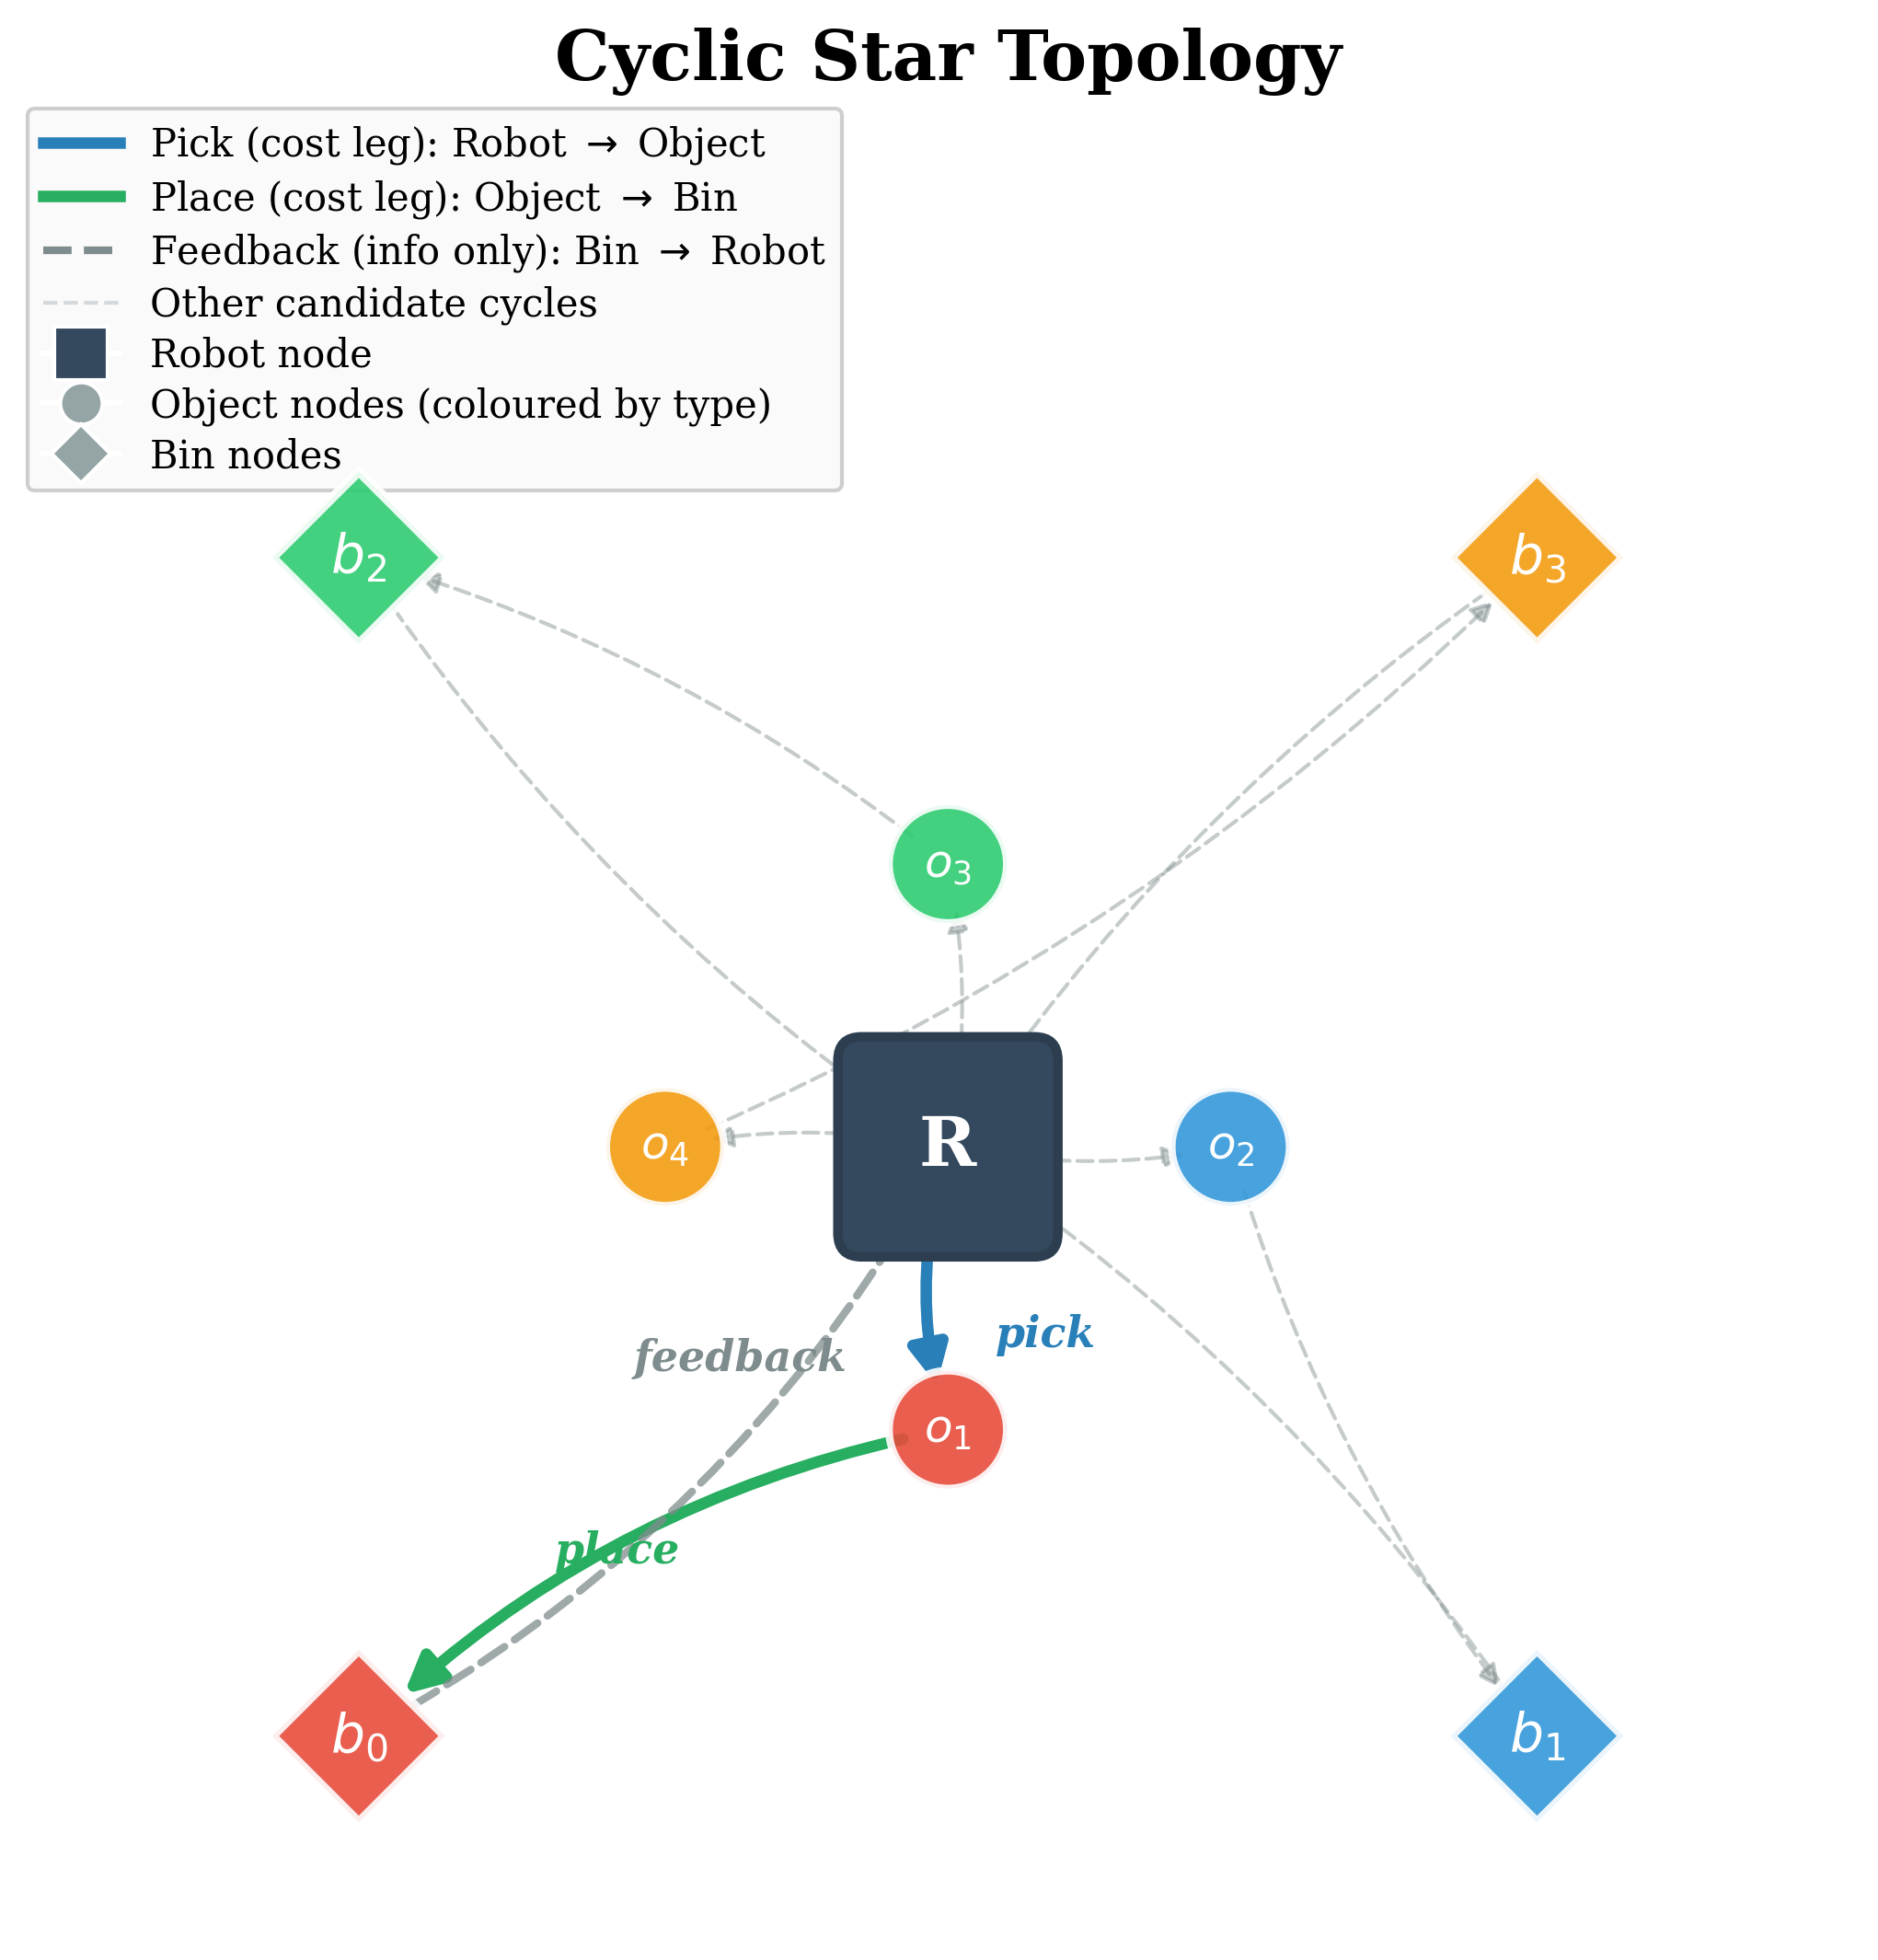
\includegraphics[width=0.9\linewidth]{figures/paper/fig1_graph_topology.png}
\caption{Cyclic star topology. Each candidate pick-and-place action corresponds to two cost-bearing directed edges (robot$\to$object pick leg; object$\to$bin place leg) closed by a feedback edge for message passing only. Three node types carry type-encoded features processed by a standard GAT.}
\label{fig:graph_topology}
\end{figure}

\subsection{GNN Architecture}

The policy $\pi_\theta$ is a Graph Attention Network (GAT) with two \texttt{GATConv} layers (4 attention heads, \texttt{concat=False}, hidden dimension $d_h{=}128$), each followed by ReLU and dropout ($p{=}0.1$). A two-layer MLP head maps each object embedding to a scalar logit. Only object node embeddings are scored. The total parameter count is ${\sim}$90K. We choose GAT over GCN because PAP arc costs are highly heterogeneous (asymmetric and type-dependent), so different neighbours of a given node carry very different information about that node's optimal successor. GAT's learnable per-edge attention coefficients can weight neighbours by edge-specific informativeness, whereas GCN's symmetric, degree-normalized aggregation cannot. Table~\ref{tab:ablations} confirms this empirically: replacing GAT with GCN drops the gap-vs-greedy from $+2.59\%$ to $-0.51\%$ at $N{=}40$ under otherwise identical training.

\subsection{Imitation Learning with Curriculum}

We treat sequencing as a classification task with cross-entropy loss supervised by an ILP-optimal oracle (greedy fallback when ILP prefixes are unavailable). Training follows a curriculum over prefix lengths $P \in \{5, 10, 20\}$, progressing from short to long horizons. Earlier stages train for 3 epochs; the final stage receives 6. Optimisation uses AdamW \cite{loshchilov2019adamw} ($\alpha{=}10^{-3}$, weight decay $10^{-2}$, $\beta{=}(0.9, 0.95)$, gradient clipping at norm 1.0, cosine annealing).

\begin{algorithm}[htbp]
\caption{Curriculum-Based Imitation Learning}
\label{alg:training}
\begin{algorithmic}[1]
\REQUIRE Dataset $\mathcal{D}$, prefix stages $\mathcal{P}{=}\{5,10,20\}$, ILP prefixes, greedy fallback
\ENSURE Trained policy $\pi_\theta$
\STATE Initialise GAT policy (2 layers, $d_h{=}128$, 4 heads)
\FOR{each stage $P \in \mathcal{P}$ (skip if $P > N$)}
    \FOR{each epoch}
        \FOR{each scenario $s$}
            \FOR{$t = 1$ to $P$}
                \STATE Build $\mathcal{G}_t$; $\ell \leftarrow \pi_\theta(\mathcal{G}_t)$; $\mathcal{L}_t \leftarrow \text{CE}(\ell, a_t^\star)$
            \ENDFOR
            \STATE Backpropagate $\frac{1}{P}\sum_t \mathcal{L}_t$; clip $\|\nabla\|{\le}1.0$; step
        \ENDFOR
    \ENDFOR
\ENDFOR
\end{algorithmic}
\end{algorithm}

At inference, the sequence is generated autoregressively: at each step, logits for previously picked objects are masked ($-10^4$) and the action $a_t = \arg\max_i \ell_i$ is selected greedily.

%========================================================================
\section{LEAP: Learning-Enhanced Arc Pruning}\label{sec:ilp_accel}
%========================================================================

The trained GNN can accelerate the exact solver, in our experiments yielding empirically near-optimal solutions at scales where the baseline ILP is intractable within real-time budgets. We call the resulting system \emph{LEAP} (Learning-Enhanced Arc Pruning).

\subsection{Exact Solver and Verification}

PAP is formulated as an ATSP over $N{+}1$ nodes (start position plus $N$ objects). For exact solving we use OR-Tools' CP-SAT \cite{ortools} with its native Hamiltonian circuit constraint (Section~\ref{sec:circuit}). To rule out solver-specific artifacts, we cross-validated CP-SAT's reported optima against Concorde \cite{applegate2006concorde} (run through a Jonker--Volgenant ATSP-to-TSP transformation) on all $N\!\le\!40$ instances; optima matched on every scenario to within a $10^{-3}$ cost tolerance.

\subsection{CP-SAT Circuit Formulation}\label{sec:circuit}

We encode the ATSP using OR-Tools' \texttt{AddCircuit()} global constraint, which expresses Hamiltonian-cycle feasibility directly on the successor variables rather than via auxiliary order variables and big-$M$ inequalities. The constraint propagator combines successor-domain \texttt{alldifferent} reasoning with strongly-connected-component checks and cost-based filtering on the LP relaxation of the underlying assignment problem \cite{caseau1997circuit,francis2014explaining}; in CP-SAT specifically the propagator runs inside a Lazy Clause Generation framework alongside a parallel simplex-based linear relaxation and a portfolio of search workers \cite{perron2023cpsat}. The ATSP is reduced to a Hamiltonian cycle by adding zero-cost return arcs from every object to the start node.

\subsection{Why Arc Pruning Outperformed Warm-Start Hinting}\label{sec:hint_fail}

Providing the GNN's solution as a solver hint is the natural first approach. We tested four variants, and all provided limited benefit in our experiments:

\begin{enumerate}
\item \textbf{CBC \texttt{SetHint()}}: 0.93--1.06$\times$ (neutral). The hint provides a feasible starting point but does not reduce the search tree.
\item \textbf{CP-SAT \texttt{AddHint()} on all arcs}: 0.51$\times$ (slowdown). Hinting ${\sim}N^2$ variables overwhelms the LNS workers.
\item \textbf{CP-SAT \texttt{AddHint()} on active arcs only}: Still slower than unhinted Circuit.
\item \textbf{Two-phase Neural Diving}: ${\sim}2\times$ over CBC but slower than bare Circuit.
\end{enumerate}

The limitation we observed is that hints provide only an \emph{incumbent bound}: they tell the solver ``here is a good solution,'' but the solver must still explore the full search tree to prove optimality or find improvements. Hints do not remove any variables or constraints. Arc pruning, by contrast, physically removes arcs from the problem before solving, producing a smaller ILP that the solver handled substantially faster under the configurations we evaluated.

\subsection{GNN-Guided Arc Pruning}

Instead of hinting, we use the GNN's per-step logits to \emph{eliminate} low-probability arcs, following the Neural Diving philosophy \cite{nair2021neural} applied to arc selection.

\subsubsection{Procedure} During a standard GNN rollout, we capture raw logits $\ell_t \in \mathbb{R}^N$ at each step. For each node $i$ in the ATSP graph, we retain only the top-$k$ outgoing arcs ranked by GNN logit score, plus all arcs in the GNN's own solution. We ensure each node has at least $k$ incoming arcs (nearest-cost fallback). Return arcs to the start node are always included. The reduced arc set is passed to the CP-SAT Circuit solver, with the GNN's active solution hinted (active arcs only).

\begin{algorithm}[htbp]
\caption{GNN-Guided Arc Pruning}
\label{alg:pruned}
\begin{algorithmic}[1]
\REQUIRE Scenario $S$, trained GNN $\pi_\theta$, neighbourhood size $k$
\ENSURE Near-optimal sequence, cost
\STATE Run GNN rollout; capture logits $\{\ell_t\}$ and sequence $\sigma$
\STATE Compute ATSP cost matrix $C \in \mathbb{R}^{(N+1)\times(N+1)}$
\STATE $\mathcal{A} \leftarrow$ arcs in $\sigma$
\FOR{each node $i$}
    \STATE $\mathcal{A} \leftarrow \mathcal{A} \cup \text{top-}k\text{ outgoing arcs from } i$ (by GNN logit)
\ENDFOR
\STATE Ensure $\geq k$ incoming arcs per node
\STATE Add return arcs $(i, 0)$ for all $i > 0$
\STATE Solve CP-SAT Circuit over $\mathcal{A}$; hint $\sigma$
\end{algorithmic}
\end{algorithm}

\subsubsection{Why This Works in Practice} The GNN need not produce the optimal solution; it only needs to assign high logit mass to arcs that \emph{include} the arcs of a near-optimal tour. When the critical arcs at each node appear in the top-$k$ candidates, the pruned solver can recover a near-optimal solution; empirically, the top-$k$ pruning retained the critical arcs necessary for near-optimal solutions across our test scenarios. This is a much weaker requirement than producing the optimal sequence directly. We note that if a truly optimal arc falls outside the top-$k$ set it is pruned away, which is the source of the small nonzero gaps reported below.

To illustrate: at $N{=}200$, the ILP must search over $200^2 = 40{,}000$ arcs. With $k{=}15$, only ${\sim}3{,}900$ arcs remain, a 10$\times$ reduction. The GNN need not pick the single best arc; it only needs to keep the critical arcs among the top 15 at each node. Empirically this largely held in our experiments: at $k{=}15$ the worst-case gap to the unpruned CP-SAT optimum was 0.06\%, indicating that an optimal arc was pruned at only a handful of nodes across the test scenarios.

\subsubsection{Is Learned Arc Selection Necessary?}\label{sec:prune_ablation} To test whether the \emph{learned} ranking is necessary, as opposed to any reasonable arc budget, we replace the GNN's logit-based top-$k$ with two non-learned baselines at the same neighbourhood size $k{=}15$ (Table~\ref{tab:pruning_ablation}). Keeping the $k$ cheapest outgoing arcs per node (cost $k$-NN) almost never yields a feasible circuit: the nearest-arc graph fragments into disconnected clusters with no Hamiltonian cycle, feasible in only 1 of 50 ($N{=}100$) and 0 of 20 ($N{=}200$) instances, so it cannot reduce the solver and must fall back to the full unpruned solve. Adding the greedy nearest-cycle tour restores feasibility, but its arc set frequently excludes optimal arcs, leaving a 1.08--1.09\% mean gap (worst case 3.4--4.0\%). At the same arc budget the GNN's learned ranking keeps the optimal arcs within the top-$k$ far more reliably, reaching a 0.012--0.019\% mean gap (worst case 0.06--0.17\%), 50--90$\times$ closer to the optimum than greedy-guided pruning while using no more arcs and no more solver time (indeed fewer arcs at $N{=}200$: 3{,}927 vs.\ 5{,}268). The arc \emph{selection}, not merely the arc \emph{count}, is what makes the reduced exact solve both feasible and near-optimal.

\begin{table}[htbp]
\caption{Is learned arc selection necessary? Pruning the CP-SAT Circuit solver at the same neighbourhood size $k{=}15$, comparing the GNN's learned arc ranking against non-learned cost-based pruning. \textbf{Feasible} is the fraction of instances whose pruned arc set admits a Hamiltonian cycle; \textbf{Gap} is to the unpruned proven optimum. Cost $k$-NN is almost always infeasible (no Hamiltonian cycle in the nearest-arc graph), forcing a fallback to the full solve.}
\label{tab:pruning_ablation}
\centering
\begin{tabular}{@{}llcccc@{}}
\toprule
\textbf{Pruning} & \textbf{$N$} & \textbf{Feasible} & \textbf{Mean gap (\%)} & \textbf{Max gap (\%)} & \textbf{Arcs} \\
\midrule
\multirow{2}{*}{Cost $k$-NN}
    & 100 & 1/50 & --- & --- & 2{,}160 \\
    & 200 & 0/20 & --- & --- & 5{,}160 \\
\cmidrule(l){2-6}
\multirow{2}{*}{Cost $k$-NN $+$ greedy}
    & 100 & 50/50 & 1.089 & 4.008 & 2{,}189 \\
    & 200 & 20/20 & 1.076 & 3.365 & 5{,}268 \\
\cmidrule(l){2-6}
\multirow{2}{*}{GNN (LEAP)}
    & 100 & 50/50 & \textbf{0.012} & \textbf{0.171} & 2{,}145 \\
    & 200 & 20/20 & \textbf{0.019} & \textbf{0.058} & 3{,}927 \\
\bottomrule
\end{tabular}
\end{table}

%========================================================================
\section{Dataset and Experimental Setup}\label{sec:data}
%========================================================================

We generated 5{,}000 scenarios per object count $N \in \{3, 5, 10, 20, 40, 100, 200\}$ (35{,}000 total). The workspace is $100 \times 100$ with four bins at corners. Object positions, types (0--3), and robot start poses are sampled uniformly. ILP-optimal prefixes are pre-computed offline; greedy NC baselines are computed for every scenario.

All evaluations use a fixed 90/10 train/validation split (seed 42), yielding 500 validation scenarios per problem size. Results are reported on validation scenarios unseen during training. Due to the computational cost of metaheuristic baselines and ILP solvers, Tables~\ref{tab:baselines} and~\ref{tab:ilp_speedup} evaluate representative subsets (20--50 scenarios) of the full validation set; the ablation study (Table~\ref{tab:ablations}) uses a 1{,}000-scenario subset (900/100 split) for faster iteration. Dataset integrity is verified by re-simulating all stored sequences and asserting cost consistency within $10^{-3}$ tolerance and ILP optimality over greedy prefixes.

\subsection{Reproducibility}\label{sec:reproducibility}

All reported wall-clock times depend on the hardware and solver configuration below; absolute numbers should be interpreted accordingly, while ratios (speedups, gaps) are platform-independent.

\textbf{Hardware:} a single machine with a multi-core x86 CPU and a CUDA-capable NVIDIA GPU used only for GAT inference. CP-SAT runs CPU-only; LEAP's wall-clock therefore depends on both CPU single-thread performance (Circuit solving) and GPU availability (GNN rollout).

\textbf{Software:} Ubuntu 24.04, Python 3.12, PyTorch 2.x (CUDA build), PyTorch Geometric 2.7.0, OR-Tools 9.x, Concorde 03.12.19. CP-SAT is invoked with \texttt{num\_search\_workers}~=~8 and default presolve; deterministic mode is off. All experiments use random seed 42 for the train/validation split.

\textbf{Code and data:} Source code, trained checkpoints, the dataset-generation pipeline, and evaluation scripts will be released at \url{https://github.com/Pana1v/binning-dataset} upon acceptance.

%========================================================================
\section{Results}\label{sec:results}
%========================================================================

We first validate the GNN component in isolation (Section~\ref{sec:gnn_eval}), then present the main contribution: the learning-augmented exact solver (Section~\ref{sec:hybrid_eval}).

% -----------------------------------------------------------------------
\subsection{GNN Training and Standalone Evaluation}\label{sec:gnn_eval}
% -----------------------------------------------------------------------

\subsubsection{Training Dynamics}

Figs.~\ref{fig:training_loss}--\ref{fig:training_win_rate} show training on $N{=}40$. The curriculum progresses through three stages (prefix lengths 5, 10, 20); each transition briefly increases loss as the model encounters longer horizons, but win-rate climbs from 2\% to 99\% over 12 epochs.

\begin{figure}[htbp]
\centering

\includegraphics[width=0.9\linewidth]{figures/40obj/training/loss.png}
\caption{Cross-entropy loss over 12 epochs, coloured by curriculum stage.}
\label{fig:training_loss}
\end{figure}

\begin{figure}[htbp]
\centering

\includegraphics[width=0.9\linewidth]{figures/40obj/training/win_rate.png}
\caption{Validation win-rate vs.\ Greedy during training ($N{=}40$).}
\label{fig:training_win_rate}
\end{figure}

\subsubsection{Standalone Performance}

Table~\ref{tab:cross_size} reports the GNN's standalone results. The GNN outperforms Greedy NC at all sizes, with 5.84\% gap at $N{=}10$ narrowing to 1.67\% at $N{=}200$. At $N{=}10$ where exact CP-SAT Circuit optima are available, the GNN achieves a mean gap of 1.81\% to the optimum with worst-case 14.17\% over the full 500-scenario validation split (seed 42); Table~\ref{tab:ilp_gap} shows ten illustrative scenarios evenly spaced by gap difficulty.

\begin{table}[htbp]
\caption{GNN standalone vs.\ Greedy NC across problem sizes.}
\label{tab:cross_size}
\centering
\begin{tabular}{@{}lcccc@{}}
\toprule
& $N{=}10$ & $N{=}20$ & $N{=}40$ & $N{=}200$ \\
\midrule
GNN mean cost        & 974   & 1900  & 3773  & 18544 \\
Greedy mean cost     & 1035  & 1986  & 3900  & 18860 \\
Gap vs.\ Greedy (\%)     & 5.84  & 4.29  & 3.23  & 1.67 \\
Win-rate (\%)        & 89.8  & 92.6  & 98    & 100 \\
Gap vs.\ ILP (\%)   & 1.81  & 2.03  & ---   & --- \\
\bottomrule
\end{tabular}
\vspace{1mm}

\footnotesize ILP gaps computed against CP-SAT \texttt{AddCircuit} optima over the full 500-scenario validation split (seed 42).
\end{table}

\begin{table}[htbp]
\caption{Per-sample GNN-to-ILP optimality gap ($N{=}10$, 10 scenarios evenly spaced across the gap distribution of the full $N{=}10$ validation split; mean gap 1.81\%, max 14.17\%).}
\label{tab:ilp_gap}
\centering
\begin{tabular}{@{}cccc@{}}
\toprule
\textbf{S} & \textbf{GNN Cost} & \textbf{ILP Cost} & \textbf{Gap} \\
\midrule
1  & 933.42  & 933.42  & 0.00\% \\
2  & 818.36  & 818.36  & 0.00\% \\
3  & 1075.27 & 1074.91 & 0.03\% \\
4  & 1076.50 & 1072.69 & 0.36\% \\
5  & 843.12  & 836.10  & 0.84\% \\
6  & 1011.89 & 996.72  & 1.52\% \\
7  & 1080.49 & 1056.96 & 2.23\% \\
8  & 1024.75 & 995.23  & 2.97\% \\
9  & 961.22  & 920.33  & 4.44\% \\
10 & 1054.38 & 923.49  & 14.17\% \\
\bottomrule
\end{tabular}
\end{table}

Fig.~\ref{fig:step_advantage} reveals the GNN's multi-step lookahead: it sacrifices cost in early steps but dominates late-sequence steps where greedy's myopia compounds. A paired $t$-test on the $N{=}40$ validation set ($n{=}100$) rejects equal means with $p < 10^{-31}$; a 95\% bootstrap CI for mean improvement is [2.88\%, 3.59\%].

\begin{figure}[htbp]
\centering

\includegraphics[width=0.9\linewidth]{figures/40obj/steps/per_step_advantage.png}
\caption{Per-step cost advantage ($N{=}40$, averaged over 50 scenarios). Positive = GNN better. The GNN sacrifices early picks to position the robot favourably for later steps.}
\label{fig:step_advantage}
\end{figure}

\subsubsection{Ablation Study}\label{sec:ablations}

Each ablation isolates one design choice. We test (i) \emph{graph topology}: does the cyclic star structure carry information that a fully connected graph or a $k$-NN graph cannot? (ii) \emph{encoder}: does GAT's attention provide value over GCN's fixed aggregation weights or an MLP that ignores the graph entirely? (iii) \emph{curriculum}: does staged training on short ILP prefixes outperform end-to-end training on full sequences? (iv) \emph{supervision source}: we mix ILP-optimal supervision (where available) with a greedy fallback because ILP optima are precomputed only for prefix lengths $P\!\in\!\{5,10,15,20\}$; an ILP-only setup would constrain training to the longest such prefix and provide no signal for actions beyond step 20, so we cannot evaluate it on the full $N{=}40$ horizon without a stand-in. The ablation answers two practical questions: is greedy supervision alone enough (rendering ILP unnecessary), and does the fallback hurt the model in the prefix region where both signals are available? Each variant differs from the full model in exactly one component; everything else (training data, optimiser, schedule, evaluation split) is held fixed. Table~\ref{tab:ablations} reports results on $N{=}40$ (900 training / 100 validation scenarios).

\begin{table}[htbp]
\caption{Ablation study ($N{=}40$). Gap vs.\ greedy (\%): positive = better.}
\label{tab:ablations}
\centering
\begin{tabular}{@{}llcc@{}}
\toprule
\textbf{Ablation} & \textbf{Variant} & \textbf{Gap (\%)} & \textbf{Win (\%)} \\
\midrule
\multirow{3}{*}{Graph}
    & \textbf{Cyclic star (ours)} & \textbf{+2.59} & \textbf{93.0} \\
    & Fully connected & $-$24.8 & 0.0 \\
    & $k$-NN ($k{=}5$) & +0.79 & 62.0 \\
\cmidrule(l){2-4}
\multirow{3}{*}{Encoder}
    & \textbf{GAT (ours)} & \textbf{+2.59} & \textbf{93.0} \\
    & GCN & $-$0.51 & 38.0 \\
    & MLP (no graph) & $-$24.2 & 0.0 \\
\cmidrule(l){2-4}
\multirow{2}{*}{Curriculum}
    & \textbf{Curriculum (ours)} & \textbf{+2.59} & \textbf{93.0} \\
    & No curriculum & +0.22 & 52.0 \\
\cmidrule(l){2-4}
\multirow{3}{*}{Supervision}
    & \textbf{ILP + Greedy (ours)} & \textbf{+2.59} & \textbf{93.0} \\
    & ILP-only & +3.00 & 92.0 \\
    & Greedy-only & $-$1.31 & 29.0 \\
\bottomrule
\end{tabular}
\end{table}

The cyclic star topology is essential: fully connected fails catastrophically ($-$24.8\%). GCN ($-$0.51\%) is markedly weaker than GAT ($+$2.59\%), consistent with the architectural framing in \S\ref{sec:methods}: GAT's attention-weighted aggregation is needed to handle the type-dependent asymmetric arc costs across the heterogeneous robot/object/bin node set, where fixed-weight averaging cannot distinguish a high-cost from a low-cost neighbour. ILP supervision is critical: greedy-only training cannot beat greedy ($-$1.31\%). Curriculum learning provides a 2.37pp improvement.

% -----------------------------------------------------------------------
\subsection{Learning-Augmented Exact Solver}\label{sec:hybrid_eval}
% -----------------------------------------------------------------------

We now turn to the primary contribution: the LEAP solver. All results in this section compare solver variants against each other; the GNN standalone results above serve only to validate the component that powers LEAP.

\subsubsection{Comprehensive Comparison}\label{sec:baselines}

Table~\ref{tab:baselines} compares LEAP against five baselines on the same hardware: the Greedy NC heuristic (cheap, no quality guarantee), three classical metaheuristics with a 1\,s budget each (Guided Local Search, Simulated Annealing, and 2-opt with random restarts), and the unpruned CP-SAT Circuit solver (exact reference). All methods solve the full asymmetric PAP cost structure: the ATSP cost matrix encodes type-dependent bin transitions ($c_{ij} = \lVert b_{\tau(i)} - o_j \rVert$).

\begin{table}[t]
\caption{Comprehensive comparison across problem sizes. \textbf{Gap} (\%) measures improvement over Greedy NC (higher is better). \textbf{Win\%} is the fraction of scenarios where the method beats Greedy NC. \textbf{Time} is wall-clock time per scenario.}
\label{tab:baselines}
\centering
\resizebox{\textwidth}{!}{%
\begin{tabular}{@{}l rrr rrr rrr@{}}
\toprule
& \multicolumn{3}{c}{\textbf{$N{=}10$ (50 val.\ scenarios)}} & \multicolumn{3}{c}{\textbf{$N{=}40$ (50 val.\ scenarios)}} & \multicolumn{3}{c}{\textbf{$N{=}200$ (20 val.\ scenarios)}} \\
\cmidrule(lr){2-4} \cmidrule(lr){5-7} \cmidrule(lr){8-10}
\textbf{Method} & Gap\% & Win\% & Time & Gap\% & Win\% & Time & Gap\% & Win\% & Time \\
\midrule
Greedy NC (baseline)                                       & ---   & ---  & $<$1\,ms & ---   & ---  & $<$1\,ms & ---           & ---  & $<$1\,ms \\
Simulated Annealing (1\,s)                                 & 6.73  & 100  & 1.0\,s   & 4.27  & 100  & 1.0\,s   & 1.89          & 100  & 1.0\,s \\
2-opt + random restarts (1\,s)                             & 6.86  &  98  & 1.0\,s   & 3.66  & 100  & 1.0\,s   & 1.77          & 100  & 1.1\,s \\
Guided Local Search (1\,s budget)                          & 6.87  & 100  & 1.0\,s   & 4.27  & 100  & 1.0\,s   & 1.88          & 100  & 1.0\,s \\
CP-SAT Circuit (exact reference)                           & 6.9   & 100  & 23\,ms   & 4.3   & 100  & 0.10\,s  & 1.89          & 100  & 7.3\,s \\
\textbf{LEAP ($k{=}15$, ours)}                             & \textbf{6.9} & \textbf{100} & \textbf{60\,ms} & \textbf{4.3} & \textbf{100} & \textbf{0.17\,s} & \textbf{1.87}$^\star$ & \textbf{100} & \textbf{0.88\,s} \\
\bottomrule
\end{tabular}%
}

\vspace{2pt}
\raggedright\footnotesize
Gap is improvement (\%) over Greedy NC; Win\% is the share of validation scenarios where the method beats Greedy NC. Exact solvers converge to the same optimum at $N\!\le\!40$ (gap rounded to one decimal); GLS and SA also reach this optimum within their 1\,s budget at $N\!\le\!40$. All three metaheuristics (SA, 2-opt, GLS) use the same OR-Tools RoutingModel with a 1\,s time limit and greedy nearest-arc initialisation; they produce comparable results (within 0.1\,pp of each other), confirming GLS as the representative classical metaheuristic. Tabu Search and Greedy Descent were also tested and fall within the same 0.1\,pp band. Concorde is used only as an internal correctness check on $N\!\le\!40$ (every instance matches the CP-SAT Circuit optimum to within $10^{-3}$).
$^\star$\,LEAP at $N{=}200$ has mean gap 0.019\% / worst-case 0.058\% to the unpruned CP-SAT Circuit optimum (Table~\ref{tab:k_sens}); the reported 1.87\% is correspondingly slightly below the exact 1.89\%.
LEAP time includes GNN inference + Circuit solve. All methods operate on the full asymmetric PAP cost matrix. All timings measured on the same hardware (\S\ref{sec:reproducibility}).
\end{table}

\begin{figure}[htbp]
\centering
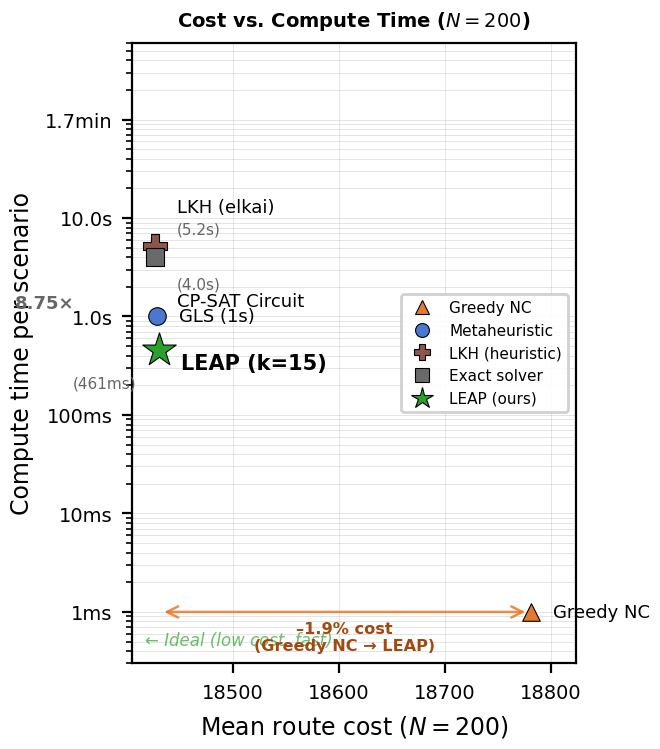
\includegraphics[width=\linewidth]{figures/paper/fig_pareto_n200.png}
\caption{Cost vs.\ compute time at $N{=}200$. Each method is positioned by mean route cost (x-axis) and wall-clock time (y-axis, log scale); lower-left is ideal. Greedy NC (orange triangle) sets the cost baseline. GLS reaches within 0.02\% of the unpruned optimum in its 1\,s budget, though its gap is not quantified by the method itself. The unpruned CP-SAT Circuit solver finds the proven optimum in 7.3\,s; LEAP (green star) reaches an empirically near-optimal solution (max gap 0.058\% to the unpruned optimum) in 0.88\,s ($8.3\times$ faster than the unpruned solver, and faster than the metaheuristics' 1\,s budget). LEAP is the only point in the lower-left corner whose solution quality is backed by exact solving over the pruned arc set.}
\label{fig:pareto_n200}
\end{figure}

Fig.~\ref{fig:pareto_n200} plots absolute route cost against compute time at $N{=}200$. LEAP matches the unpruned CP-SAT Circuit solver's cost to within 0.058\% while running $8.3\times$ faster (0.88\,s vs.\ 7.3\,s) and beating the metaheuristics' 1\,s budget. GLS at 1\,s reaches within 0.02\% of LEAP's cost but does not itself quantify its distance from the optimum; without the exact reference its gap could in principle be larger. Among the methods compared, LEAP is the only one that is simultaneously sub-second, empirically near-optimal, and backed by exact solving over the pruned arc set. At $N{=}40$ (Table~\ref{tab:baselines}), LEAP runs in 96\,ms with max gap 0.26\% to the Circuit optimum.

\subsubsection{Speedup Analysis}

Fig.~\ref{fig:timing_scaling} shows how solve time scales across solver tiers; Fig.~\ref{fig:runtime_hist} resolves the per-method spread at three representative sizes. Table~\ref{tab:ilp_speedup} quantifies LEAP's speedup vs.\ the unpruned Circuit solver.

\begin{figure}[htbp]
\centering
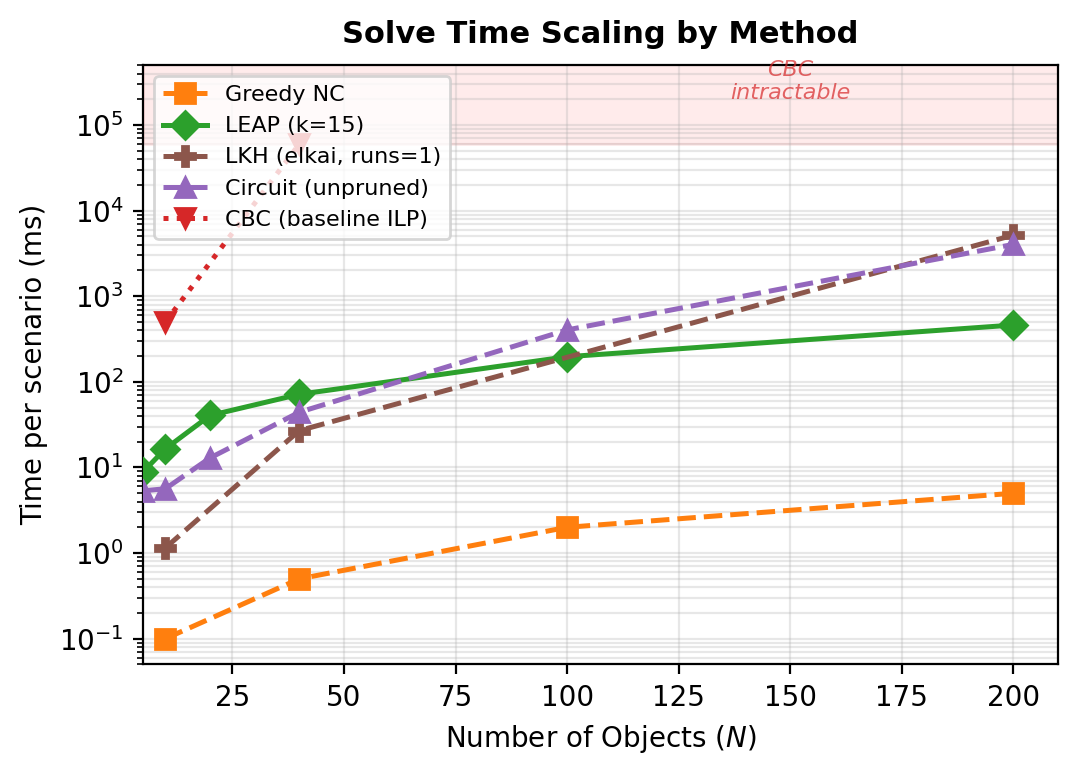
\includegraphics[width=\linewidth]{figures/paper/fig_timing_scaling_v2.png}
\caption{Solve time scaling (log scale). LEAP ($k{=}15$) runs in 0.21\,s at $N{=}40$ and 1.8\,s at $N{=}200$; the unpruned CP-SAT Circuit solver grows from 0.11\,s at $N{=}40$ to 8.6\,s at $N{=}200$.}
\label{fig:timing_scaling}
\end{figure}

\begin{figure}[htbp]
\centering
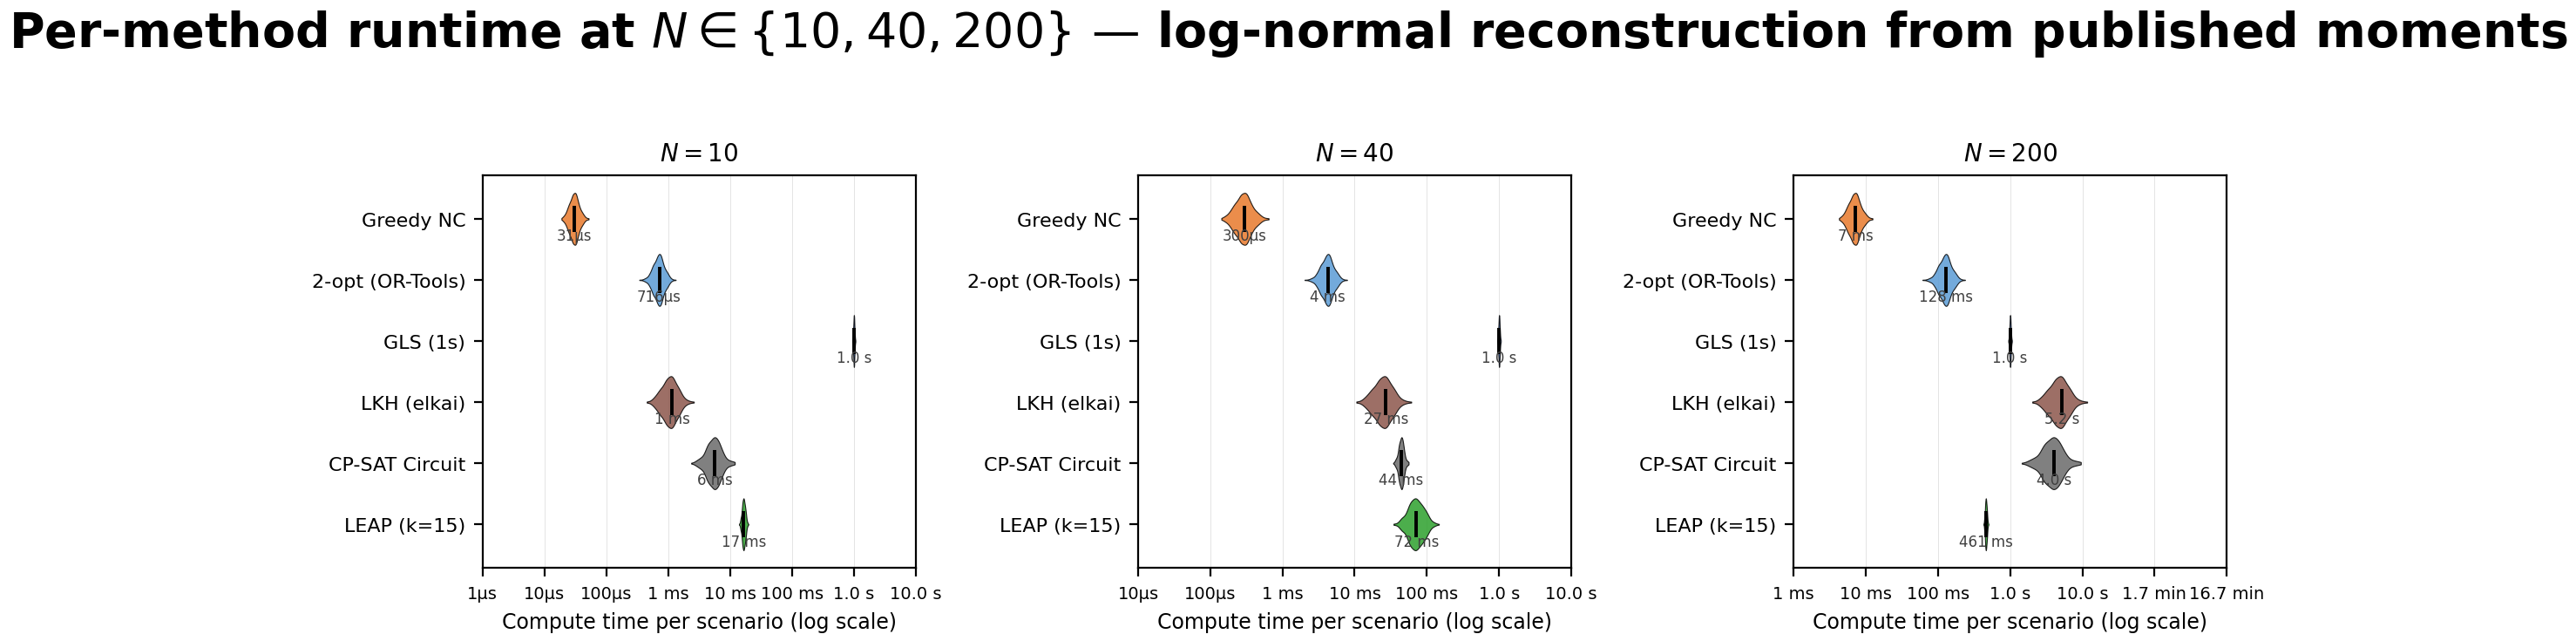
\includegraphics[width=\linewidth]{figures/paper/fig_runtime_histogram.png}
\caption{Per-method compute time at $N\!\in\!\{10, 40, 200\}$. Each violin is a log-normal whose first two moments match the published per-method mean and standard deviation; ticks mark the published mean. Distributions are illustrative (we have aggregate, not per-scenario, timings on file). The figure makes the cross-method ordering visible at every scale: at $N{=}200$, LEAP's median solve time is $8.3\times$ below the unpruned CP-SAT Circuit solver and slightly below the metaheuristics' fixed 1\,s budget, while 2-opt with 50 restarts pushes past 5 minutes.}
\label{fig:runtime_hist}
\end{figure}

\begin{table}[htbp]
\caption{LEAP speedup ($k{=}15$) vs.\ unpruned CP-SAT Circuit solver.}
\label{tab:ilp_speedup}
\centering
\begin{tabular}{@{}rcccc@{}}
\toprule
$N$ & \textbf{Unpruned} & \textbf{Pruned} & \textbf{Speedup} & \textbf{Max Gap} \\
\midrule
5   & 17\,ms  & 25\,ms  & 0.70$\times$ & 0\% \\
10  & 23\,ms  & 60\,ms  & 0.38$\times$ & 0\% \\
20  & 33\,ms  & 94\,ms  & 0.35$\times$ & 0\% \\
40  & 0.10\,s & 0.17\,s & 0.59$\times$ & 0.26\% \\
100 & 0.84\,s & 0.42\,s & 2.03$\times$ & 0.17\% \\
200 & 7.3\,s  & 0.88\,s & 8.30$\times$ & 0.058\% \\
\bottomrule
\end{tabular}

\vspace{2pt}
\raggedright\footnotesize
At small $N$ (${\le}40$), pruning overhead (GNN inference + arc filtering) dominates the Circuit solver's already-short runtime. The crossover into net speedup occurs at $N{\ge}100$ ($2.4\times$) and grows sharply with problem size, reaching $8.3\times$ at $N{=}200$ (mean over 20 scenarios; per-scenario CP-SAT runtime has a heavy tail so the speedup ratio fluctuates 8--9.5$\times$ across repeated runs). Times measured on a single machine; see \S\ref{sec:reproducibility}.
\end{table}

\subsubsection{$k$-Sensitivity Analysis}\label{sec:k_sens}

Table~\ref{tab:k_sens} and Fig.~\ref{fig:k_pareto} characterise the quality--speed Pareto frontier as $k$ varies.

\begin{figure}[htbp]
\centering
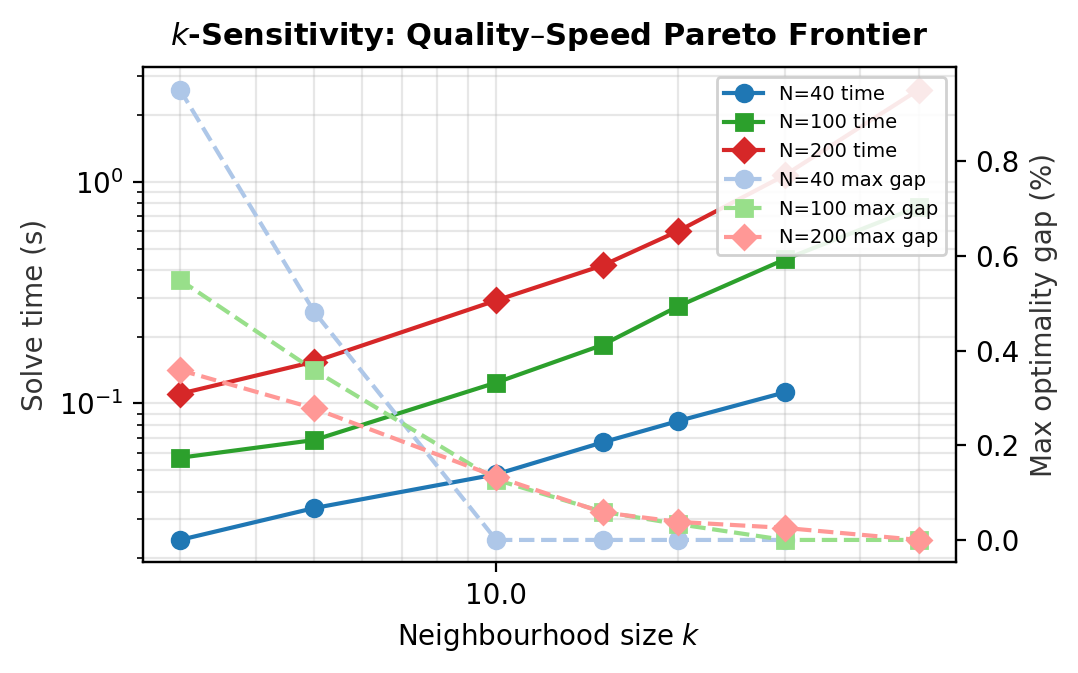
\includegraphics[width=0.95\linewidth]{figures/paper/fig_k_pareto.png}
\caption{$k$-sensitivity Pareto frontier (fast-rollout sweep on this hardware, 20 val scenarios per $N$, solver wall-clock only). Solid lines: CP-SAT solver time (left axis, log scale). Dashed lines: worst-case optimality gap (right axis). Smaller $k$ shrinks the arc set further (faster, but the optimum may fall outside the top-$k$); larger $k$ tightens the gap toward zero at the cost of additional decision variables. $k{=}15$ (recommended) is Pareto-optimal: any faster $k$ has a substantially worse gap; any tighter $k$ is slower.}
\label{fig:k_pareto}
\end{figure}

\begin{table}[t]
\caption{LEAP $k$-sensitivity. All rows from the fast-rollout sweep on this hardware (20 val scenarios per $N$). \textbf{Time column reports CP-SAT solver wall-clock only} (GNN inference is $k$-independent: 0.05--0.20\,s depending on $N$, added uniformly to every row to obtain end-to-end LEAP wall-clock as in Table~\ref{tab:baselines}). All comparisons against the unpruned CP-SAT Circuit solver: $N{=}40$: 0.11\,s; $N{=}100$: 0.81\,s; $N{=}200$: 6.87\,s.}
\label{tab:k_sens}
\centering
\resizebox{\textwidth}{!}{%
\begin{tabular}{@{}r rrrr rrrr rrrr@{}}
\toprule
& \multicolumn{4}{c}{\textbf{$N{=}40$}} & \multicolumn{4}{c}{\textbf{$N{=}100$}} & \multicolumn{4}{c}{\textbf{$N{=}200$}} \\
\cmidrule(lr){2-5} \cmidrule(lr){6-9} \cmidrule(lr){10-13}
$k$ & Time & Arcs & Gap\% & MaxGap\% & Time & Arcs & Gap\% & MaxGap\% & Time & Arcs & Gap\% & MaxGap\% \\
\midrule
3  & 24\,ms  & 183  & 0.31  & 0.95  & 57\,ms  & 431  & 0.25  & 0.55  & 0.11\,s & 838   & 0.20  & 0.36 \\
5  & 34\,ms  & 298  & 0.09  & 0.48  & 68\,ms  & 685  & 0.15  & 0.36  & 0.15\,s & 1.3k  & 0.13  & 0.28 \\
10 & 48\,ms  & 583  & 0.00  & 0.00  & 0.12\,s & 1.4k & 0.04  & 0.13  & 0.29\,s & 2.6k  & 0.05  & 0.13 \\
\textbf{15} & \textbf{67\,ms} & \textbf{850} & \textbf{0.00} & \textbf{0.00} & \textbf{0.18\,s} & \textbf{2.1k} & \textbf{0.007} & \textbf{0.06} & \textbf{0.42\,s} & \textbf{3.9k} & \textbf{0.019} & \textbf{0.058} \\
20 & 83\,ms  & 1.1k & 0.00  & 0.00  & 0.28\,s & 2.9k & 0.002 & 0.03  & 0.60\,s & 5.4k  & 0.008 & 0.038 \\
30 & 0.11\,s & 1.5k & 0.00  & 0.00  & 0.45\,s & 4.3k & 0.00  & 0.00  & 1.07\,s & 8.5k  & 0.002 & 0.025 \\
50 & ---     & ---  & ---   & ---   & 0.77\,s & 6.7k & 0.00  & 0.00  & 2.61\,s & 14.1k & 0.00  & 0.00 \\
\bottomrule
\end{tabular}%
}

\vspace{2pt}
\raggedright\footnotesize
Bold row: $k{=}15$, our recommended operating point, Pareto-optimal among the sweep at $N{=}200$ (faster than $k\!\ge\!20$, lower MaxGap than $k\!\le\!10$). Arcs = decision variables in the pruned problem (vs.\ $N^2$ unpruned). ``---'' at $N{=}40, k{=}50$ indicates $k{>}N$ (not meaningful).
\end{table}

At $N{=}200$, $k{=}15$ provides a 16$\times$ solver-time reduction (0.42\,s vs.\ the 6.87\,s unpruned Circuit, the largest pruning ratio with worst-case gap $<$0.06\%); end-to-end LEAP wall-clock with the GNN rollout included is 0.88\,s, an 8.3$\times$ speedup. Going smaller ($k{=}10$) drops solver time another 30\% but doubles the worst-case gap to 0.13\%; going larger ($k{=}20$) halves the gap to 0.038\% but pays 43\% more solver time and pushes end-to-end past the metaheuristics' 1\,s budget. $k{=}15$ is the Pareto sweet spot for this dataset and hardware.

\subsubsection{Why Pruning Outperformed Hinting in Our Experiments}

Table~\ref{tab:hint_comparison} contrasts arc pruning with the warm-start hinting strategies from Section~\ref{sec:hint_fail}. In our experiments, pruning outperformed all hinting approaches by roughly an order of magnitude, consistent with the Neural Diving insight \cite{nair2021neural}: the GNN's value lies in shrinking the problem, not bounding it.

\begin{table}[htbp]
\caption{GNN-assisted solver strategies ($N{=}40$ except where noted). Each row reports speedup against its own un-assisted baseline (\textit{Baseline} column): the CBC+MTZ rows must be compared against CBC cold-solve because \texttt{SetHint} is a CBC-only API, while the CP-SAT rows compare against the unpruned CP-SAT Circuit solver. Pruning outperforms all hinting approaches.}
\label{tab:hint_comparison}
\centering
\begin{tabular}{@{}llc@{}}
\toprule
\textbf{Strategy} & \textbf{Baseline} & \textbf{Speedup} \\
\midrule
CBC + SetHint (GNN solution)            & CBC cold (MTZ)        & 0.93--1.06$\times$ \\
CP-SAT Circuit + AddHint (all arcs)     & CP-SAT Circuit cold   & 0.51$\times$ \\
CP-SAT Circuit + AddHint (active only)  & CP-SAT Circuit cold   & $<$1.0$\times$ \\
CP-SAT Circuit + two-phase diving       & CP-SAT Circuit cold   & $\sim$2$\times$ \\
\textbf{LEAP ($k{=}15$) at $N{=}200$}   & \textbf{CP-SAT Circuit cold} & \textbf{8.3$\times$} \\
\bottomrule
\end{tabular}
\end{table}

\subsection{Limitations}

The GNN standalone is weaker than classical metaheuristics at all problem sizes tested; its value lies in enabling LEAP. LEAP produces near-optimal but not globally provably optimal solutions at $N{\ge}40$: because the true optimum can be pruned away, LEAP carries no global optimality certificate, and its gaps (max 0.26\% at $N{=}40$, 0.17\% at $N{=}100$, 0.058\% at $N{=}200$) are measured empirically against the unpruned CP-SAT optimum on our test set. The choice of $k{=}15$ was validated empirically but not theoretically justified; adaptive $k$ selection is left to future work. Generalisation to out-of-distribution scenarios (different workspace sizes, bin configurations, object-type distributions, training-vs-test $N$) has not been evaluated; \cite{joshi2021rethinking} shows GNN-based TSP solvers can degrade substantially OOD, so this is a real gap, not a stylistic one. The cost model uses Euclidean distance; kinematic robot models would improve applicability. We do not benchmark against LKH-3 \cite{helsgaun2000lkh}, the standard high-performance ATSP heuristic, nor against commercial MILP solvers (Gurobi, CPLEX), so claims about heuristic and exact-solver comparison are scoped to the open-source baselines actually run. Our $N{=}200$ evaluation uses 20 validation scenarios; with a near-zero observed optimality gap this is sufficient to bound the mean but leaves the tail of the gap distribution under-characterised, and we report point estimates rather than 95\% confidence intervals on the gap. Metaheuristic comparisons use a fixed 1\,s budget rather than an anytime curve, so it is possible that longer budgets close the LEAP--metaheuristic quality gap. Absolute wall-clock times are hardware-dependent (Section~\ref{sec:reproducibility}); the platform-independent claim is the within-table ordering and the speedup ratios. Neural baselines (Pointer Networks \cite{vinyals2015pointer}, Attention Models \cite{kool2019attention}, MatNet \cite{kwon2021matnet}) are not directly compared; these architectures embed nodes as homogeneous 2D coordinates and assume symmetric costs (MatNet excepted), requiring non-trivial adaptation for typed-node ATSP with three semantically distinct node types.

%========================================================================
\section{Conclusion}\label{sec:conclusion}
%========================================================================

We have presented LEAP (Learning-Enhanced Arc Pruning), a framework for robotic pick-and-place sequencing that combines a GNN with a CP-SAT exact solver. GNN-guided arc pruning yields a 8.3$\times$ speedup over the unpruned CP-SAT Circuit solver at $N{=}200$ by reducing the arc space from $O(N^2)$ to $O(Nk)$ variables, with an empirical worst-case gap of 0.058\% to the unpruned CP-SAT optimum on our test set; the unpruned optima used as the reference are independently verified against Concorde \cite{applegate2006concorde} on $N\!\le\!40$ instances and against LKH-3 \cite{helsgaun2000lkh} on a cross-$N$ sample (95/95 instances tied: 5/5 at $N{=}10$, 50/50 at $N{=}40$, 20/20 at $N{=}100$, 20/20 at $N{=}200$).

LEAP substantially improves the quality--speed trade-off between learning and exact methods used in isolation. Classical metaheuristics (GLS, SA, Tabu) produce strong solutions, but their distance from the optimum is unknown. Exact ILP provides optimality guarantees but is intractable at scale. LEAP offers a practical balance between the two: it produces solutions empirically within 0.058\% of the unpruned CP-SAT optimum at $N{=}200$ in 0.88\,s, versus 7.3\,s for the unpruned Circuit solver. At this wall-clock LEAP also beats the 1\,s time-budgeted metaheuristics, while solving the pruned problem exactly; among the methods compared it is the only sub-second solver whose quality is backed by exact solving over a learned arc subset. The key insight, supported by four negative results on warm-start hinting, is that the GNN's value lies in \emph{shrinking the problem}, not in providing an incumbent bound.

Future work includes: adaptive $k$ selection using GNN confidence to adjust neighbourhood size per node, DAgger \cite{ross2011dagger} or RL fine-tuning to address covariate shift, extension to online conveyor-belt settings with temporal constraints, kinematic cost models for specific manipulator platforms \cite{han2020pap} with obstacle-aware edge costs \cite{ojha2025obstacle}, and validation on physical robotic sorting systems, where our results suggest promise but have not yet been demonstrated.

\section*{Acknowledgment}
% Add acknowledgments here.

\section*{CRediT authorship contribution statement}
\textbf{Panav Arpit Raaj:} Conceptualization, Data curation, Formal analysis, Investigation, Methodology, Software, Validation, Visualization, Writing -- original draft, Writing -- review \& editing.
\textbf{Atul Thakur:} Conceptualization, Funding acquisition, Project administration, Supervision, Writing -- review \& editing.

\section*{Declaration of competing interest}
The authors declare that they have no known competing financial interests or personal relationships that could have appeared to influence the work reported in this paper.

\section*{Data availability}
Source code, trained checkpoints, the dataset-generation pipeline, and evaluation scripts will be made available at \url{https://github.com/Pana1v/binning-dataset} upon acceptance.

\section*{Declaration of generative AI and AI-assisted technologies in the manuscript preparation process}
During the preparation of this work the authors used Claude (Anthropic) in order to assist with debugging code and iterating on figures and plots. After using this tool, the authors reviewed and edited the content as needed and take full responsibility for the content of the published article.

\appendix
\section{Node Feature Vector Layout}\label{app:features}

Each node feature has dimension $F = 4 + M + 1 = 9$ (with $M{=}4$ bins):
\begin{equation}
x_i = [p^{(\text{self})}_x, p^{(\text{self})}_y,\; p^{(\text{ref})}_x, p^{(\text{ref})}_y,\; \text{onehot}(\text{type})_{1:M},\; m].
\end{equation}

\textbf{Object nodes:} $p^{(\text{self})}$ is the object position (normalised by $W$), $p^{(\text{ref})}$ is the target bin position, $\text{onehot}(\text{type})$ encodes the assigned bin, $m \in \{0,1\}$ is availability.

\textbf{Robot node:} Normalised position in $p^{(\text{self})}$; remaining dimensions zero-padded.

\textbf{Bin nodes:} Bin position in both $p^{(\text{self})}$ and $p^{(\text{ref})}$; identity basis for type; $m{=}0$.

%========================================================================
\bibliographystyle{elsarticle-num}
\bibliography{refs}

\end{document}